\section{Reinforcement learning algorithm}\label{sec:reinforcement_learning}

The agent-based mode described in Section~\ref{sec:agent_based_model} describes
how the agents can interact with the environment.
The next step is to describe how the agents can learn from their interactions.
A reinforcement learning algorithm is described in this section where the agents
update their service rates based on the utilities they receive from the
queueing system~\cite{kaelbling1996, liu2019, ayesta2022}.
The concepts described in Section~\ref{sec:queueing_section} and
Section~\ref{sec:agent_based_model} are incorporated in the reinforcement
learning algorithm so that the agents decide how fast they should serve the
customers in order to maximise their own utility.

The reinforcement learning algorithm is a policy iteration
algorithm~\cite{mahadevan1996average} where the agents update their service
rates based on the utilities they receive from the queueing system.
The service rates will be referred to as the policy in this section.
A policy is a set of service rates for every server for each possible state
they can be in.
The following pseudo-code describes the reinforcement learning algorithm.
At each time step, the agent receives a utility $U$ from the queueing system
and updates its service rate $s$ based on the utility it received.
Recall from Section~\ref{sec:agent_based_model} that each agent (server) has
a different service rate for each possible state they can be in.

\vspace*{0.5cm}

\begin{lstlisting}
Choose an initial policy
Run simulation with current policy
Calculate initial utility U_current
For each time step
    1. Choose a server k
    2. Choose a state (u, v)
    3. Update policy for server k and state (u, v)
    4. Rerun simulation
    5. Calculate utility U_new
    6. If utility U is higher than previous utility
        - Update service rate s
        - Update U_current to U_new

\end{lstlisting}

The algorithm has been implemented in python and the scripts are archived and
can be found in~\cite{michalis_panayides_2023_7586860}.

The total number of time steps is a parameter that needs to be set to a high
enough value to ensure that the agents have enough time to learn from their
interactions with the queueing system.
Additionally, in order to eliminate any stochasticity from the simulation
at each time step, the simulation is run for a fixed runtime and a fixed number
of trials.
Furthermore, when choosing a new policy for a server and a state, the
algorithm will choose a new policy that is within a certain range of the
current policy and that cannot be below zero.

An additional rule is that there is a maximum service rate that a server can
have for any given state.
This is to ensure that unrealistic service rates are not chosen.
Some numeric results on why this rule is necessary are presented in
Section~\ref{sec:utility_7_no_upper_bound_results}.

Consider an example of a queueing system with \(2\) servers and the following
set of states:

\begin{equation}
    \mathcal{S} = \{(0, 0), (0, 1), (0, 2), (1, 2), (0, 3), (1, 3)\}
\end{equation}

The \(2\) servers have a different service rate for each state
\((u, v) \in \mathcal{S}\).
An initial policy is chosen where the service rates for the \(2\) servers is
set to:

\begin{equation*}
    \mu^{(1)} =
    \begin{cases}
        1 & \text{if } v < 2 \\
        1.5 & \text{otherwise}
    \end{cases}
    \qquad \qquad
    \mu^{(2)} =
    \begin{cases}
        0.8 & \text{if } v < 3 \\
        2 & \text{otherwise}
    \end{cases}
\end{equation*}

Figures~\ref{fig:reinforcement_learning_policy_exmaple_1}~-~\ref{fig:reinforcement_learning_policy_exmaple_3} show the
policy for the \(2\) servers for the first \(3\) time steps of the
reinforcement learning algorithm.

\begin{figure}[H]
    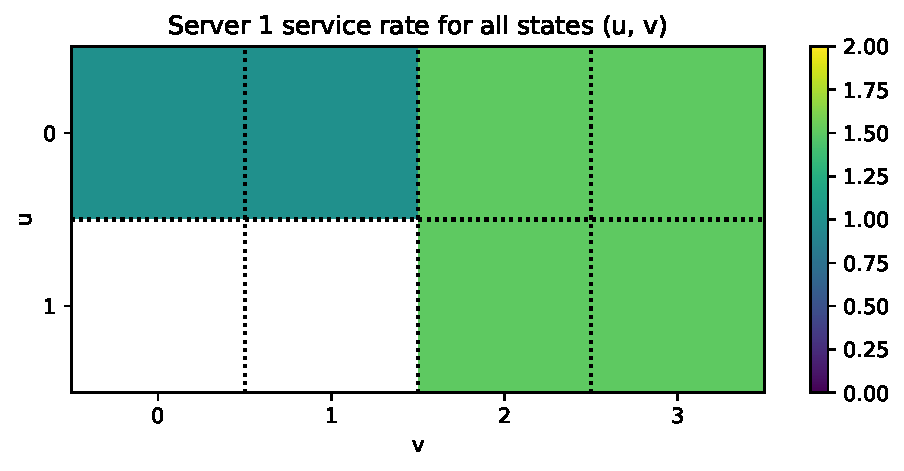
\includegraphics[width=0.45\textwidth]{chapters/06_agent_based_extension/Bin/reinforcement_learning_policy_example/server_1_1.pdf}
    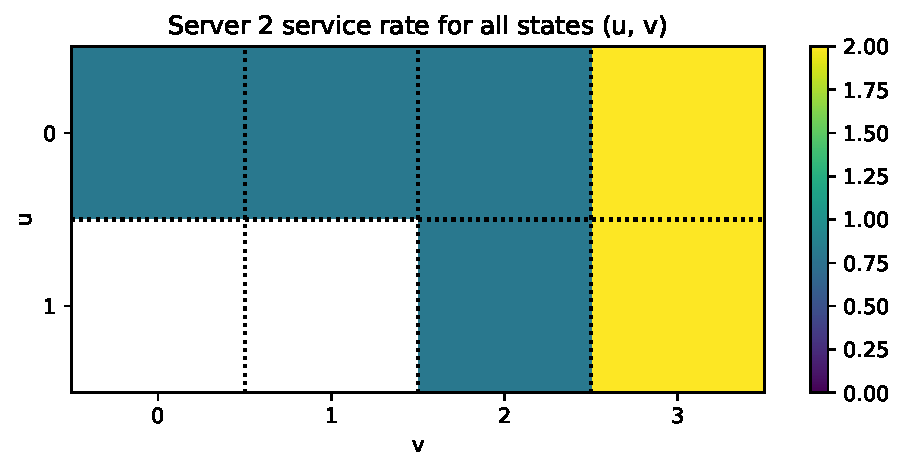
\includegraphics[width=0.45\textwidth]{chapters/06_agent_based_extension/Bin/reinforcement_learning_policy_example/server_2_1.pdf}
    \caption{Example policy for server \(1\) and server \(2\) at time step \(1\)}
    \label{fig:reinforcement_learning_policy_exmaple_1}
\end{figure}


\begin{figure}[H]
    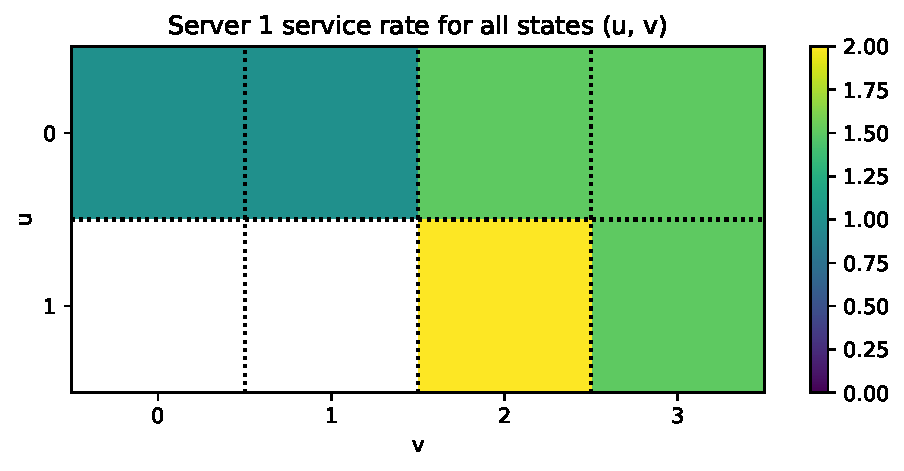
\includegraphics[width=0.45\textwidth]{chapters/06_agent_based_extension/Bin/reinforcement_learning_policy_example/server_1_2.pdf}
    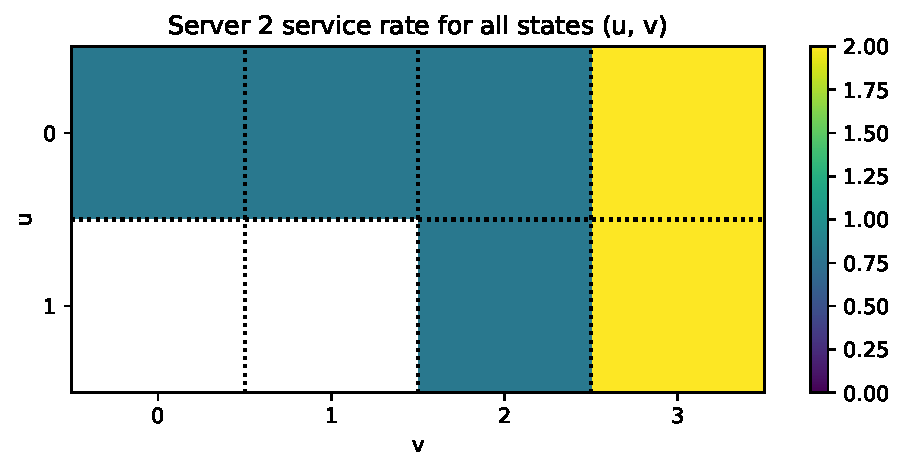
\includegraphics[width=0.45\textwidth]{chapters/06_agent_based_extension/Bin/reinforcement_learning_policy_example/server_2_2.pdf}
    \caption{Example policy for server \(1\) and server \(2\) at time step \(2\)}
    \label{fig:reinforcement_learning_policy_exmaple_2}
\end{figure}

\begin{figure}[H]
    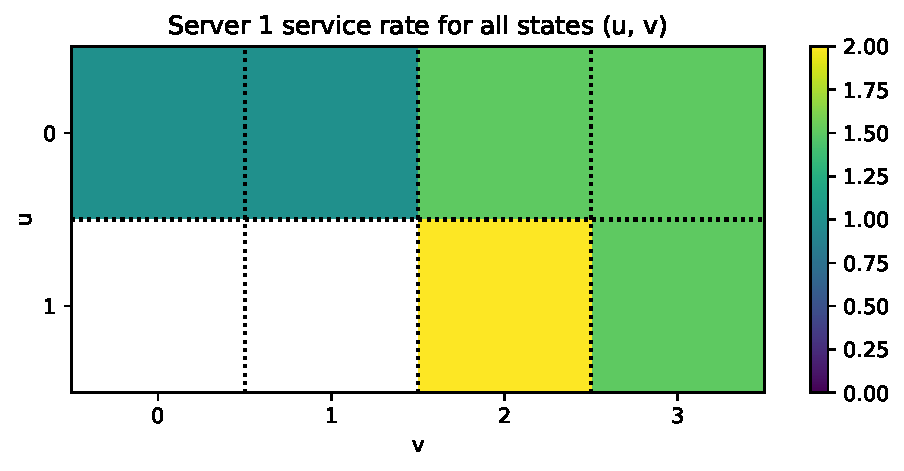
\includegraphics[width=0.45\textwidth]{chapters/06_agent_based_extension/Bin/reinforcement_learning_policy_example/server_1_3.pdf}
    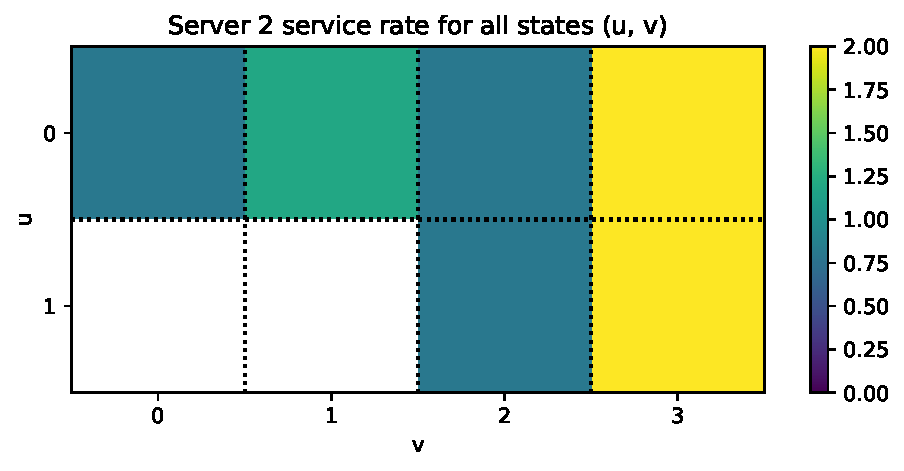
\includegraphics[width=0.45\textwidth]{chapters/06_agent_based_extension/Bin/reinforcement_learning_policy_example/server_2_3.pdf}
    \caption{Example policy for server \(1\) and server \(2\) at time step \(3\)}
    \label{fig:reinforcement_learning_policy_exmaple_3}
\end{figure}



\subsection{Numeric results}\label{sec:reiforcement_learning_numeric_results}

The reinforcement learning algorithm is implemented in python and the scripts
along with the generated data presented in this section have been archived and
can be found in~\cite{michalis_panayides_2023_7586860}.
Additional numerical experiments can also be found in
Appendix~\ref{appendix:reinforcement_learning}.

Consider a queueing system with the following parameters:

\begin{multicols}{4}
    \begin{itemize}
        \item \(\lambda_2 = 1\)
        \item \(\lambda_1 = 0.5 \)
        \item \(\mu = 0.7\)
        \item \(C = 4\)
        \item \(T = 7\)
        \item \(N = 10\)
        \item \(M = 7 \)
    \end{itemize}
\end{multicols}

Note that for the initial policy, the service rates of the \(4\) servers are
set to \(\mu = 0.7\) for all servers and all states.
In addition, the \(4\) servers are set to be of the same expertise level as
described in Section~\ref{sec:agent_based_case_study}.
That is, server \(1\) is an experienced server, server \(2\) and server
\(3\) are moderate servers and server \(4\) is an intern.
That means that when server \(1\) is not busy they will always receive the
incoming individual, otherwise either server \(2\) or server \(3\) will
receive that individual with an equal probability.
Finally, server \(4\) may serve an individual only when every other server is
busy.

The remaining of this section focuses on the results of the reinforcement
learning algorithm from using utility functions \(U_k^{(3)}\) and
\(U_k^{(7)}\) with different values of \(e\).
The two utility functions are chosen because they were considered to be the
most realistic ones.
In addition utility function \(U_k^{(7)}\) is used to express the effect of
having to balance the server's best interest with the system's best interest.
It is assumed that a server would like the proportion of individuals served
to be as high as possible, while also maximising their own idle time.
This is what utility function \(U_k^{(7)}\) aims to capture.

\subsubsection{Utility function 3 \((U_k^{(3)})\) with \(e = 0.1\)}
\label{sec:utility_3_results}

Consider utility function 3 defined in~\eqref{eq:utility_3} where
\(U_k^{(3)} = e \, \bar{m}^{(k)} + (1 - e) \, (R - B^{(k)})\).
Thus a server's utility corresponds to the weighted average of the server's
service time and their idle time.
This means that in order for servers to increase their utility they either
need to work faster or increase the amount of time they are idle.
Figure~\ref{fig:RL_utility3_1_e01} shows the utilities and mean service rate
of servers from the reinforcement learning run using utility function
\(U_k^{(3)}\) with \(e = 0.1\) and \(100,\!000\) time steps.

\begin{figure}[H]
    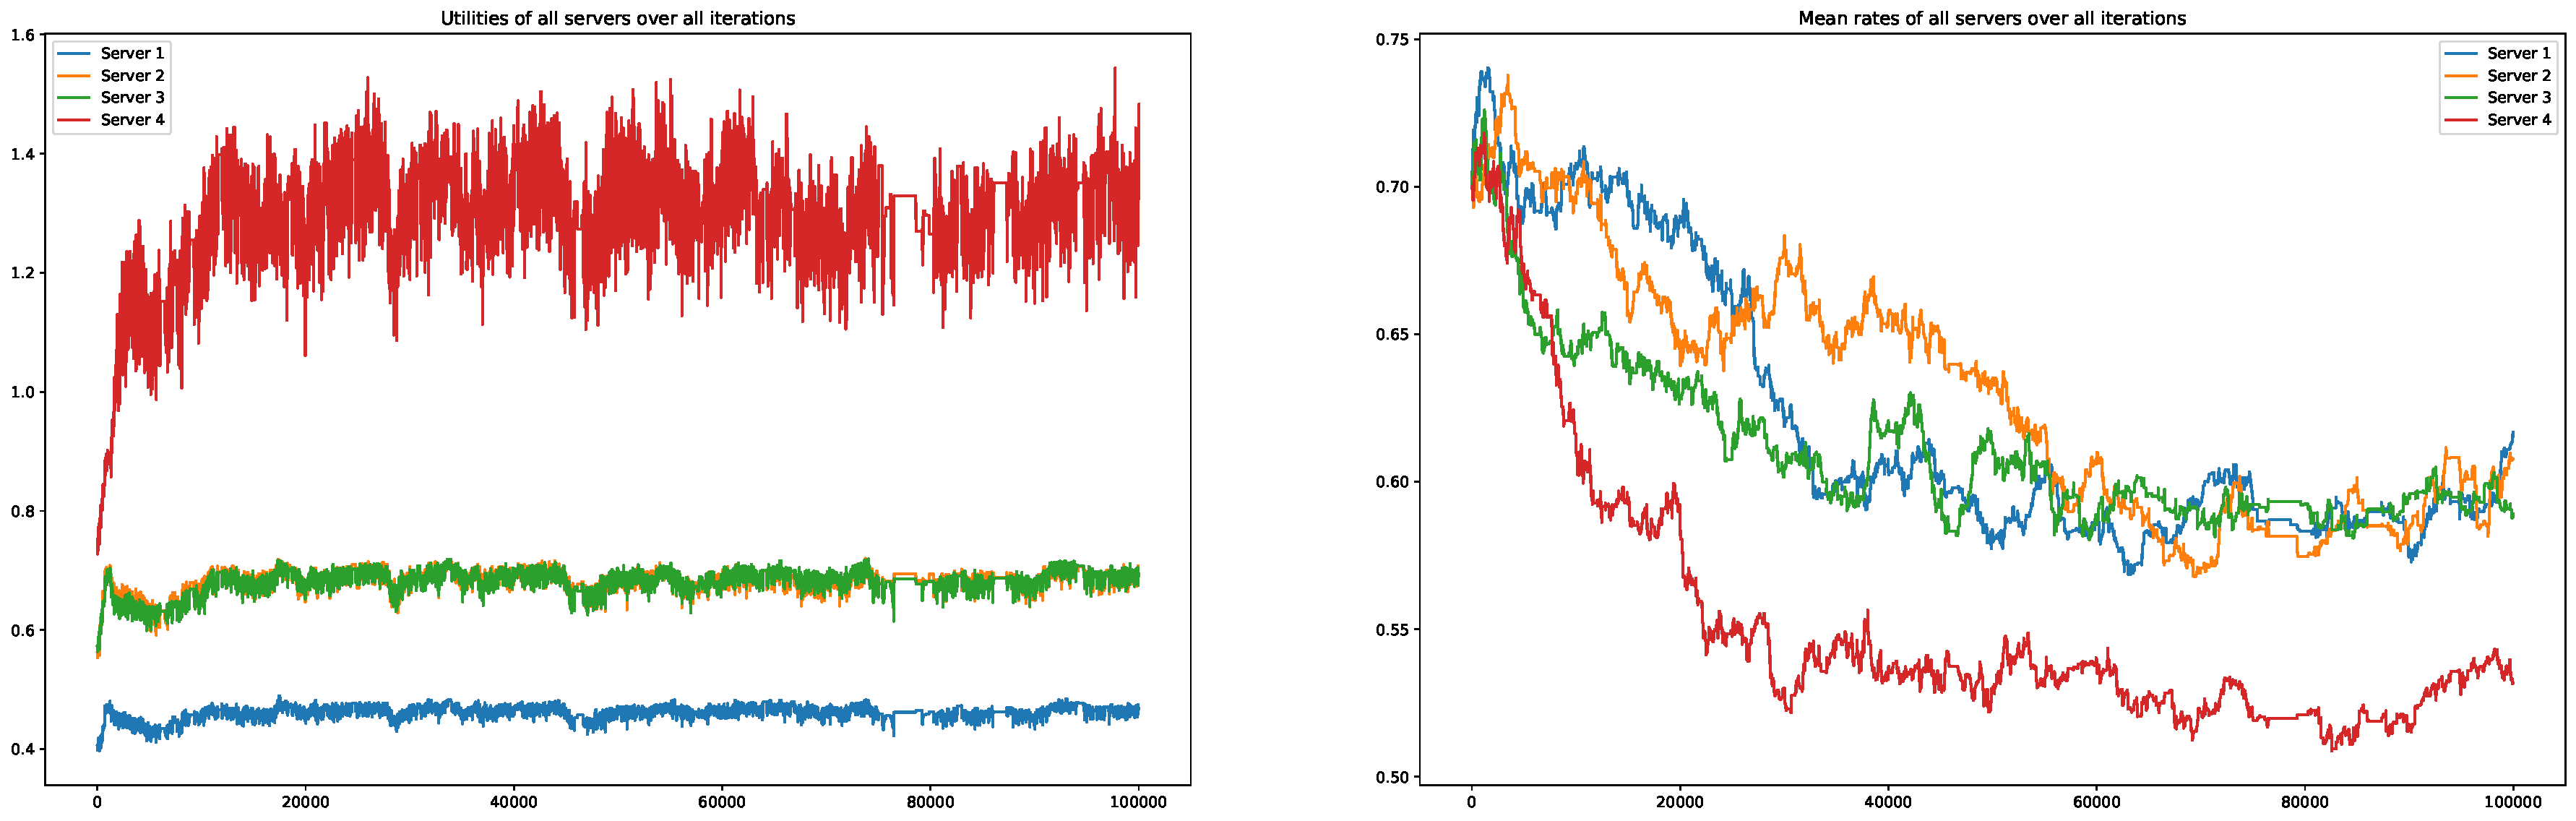
\includegraphics[width=\textwidth]{chapters/06_agent_based_extension/Bin/reinforcement_learning_results/utility_3/u3_1_e01.pdf}
    \caption{Utilities (left) and mean service rate (right) of servers from the
    reinforcement learning run using utility function \(U_k^{(3)}\) with
    \(e = 0.1\) and \(100,\!000\) time steps}
    \label{fig:RL_utility3_1_e01}
\end{figure}

It can be seen from Figure~\ref{fig:RL_utility3_1_e01} that the utility of
server \(1\) (that has the highest priority on incoming individuals) is the
lowest, while server \(4\) (that has the lowest priority on incoming)
individuals has the highest utility.
In addition, the mean service rate of server \(4\) is the lowest while servers
\(1\), \(2\) and \(3\) have similar mean service rates.
All servers managed to increase their utility by reducing their mean service
rate (i.e. working faster).
Figure~\ref{fig:RL_utility3_2_e01} shows the same example as above but with
\(500,\!000\) time steps.

\begin{figure}[H]
    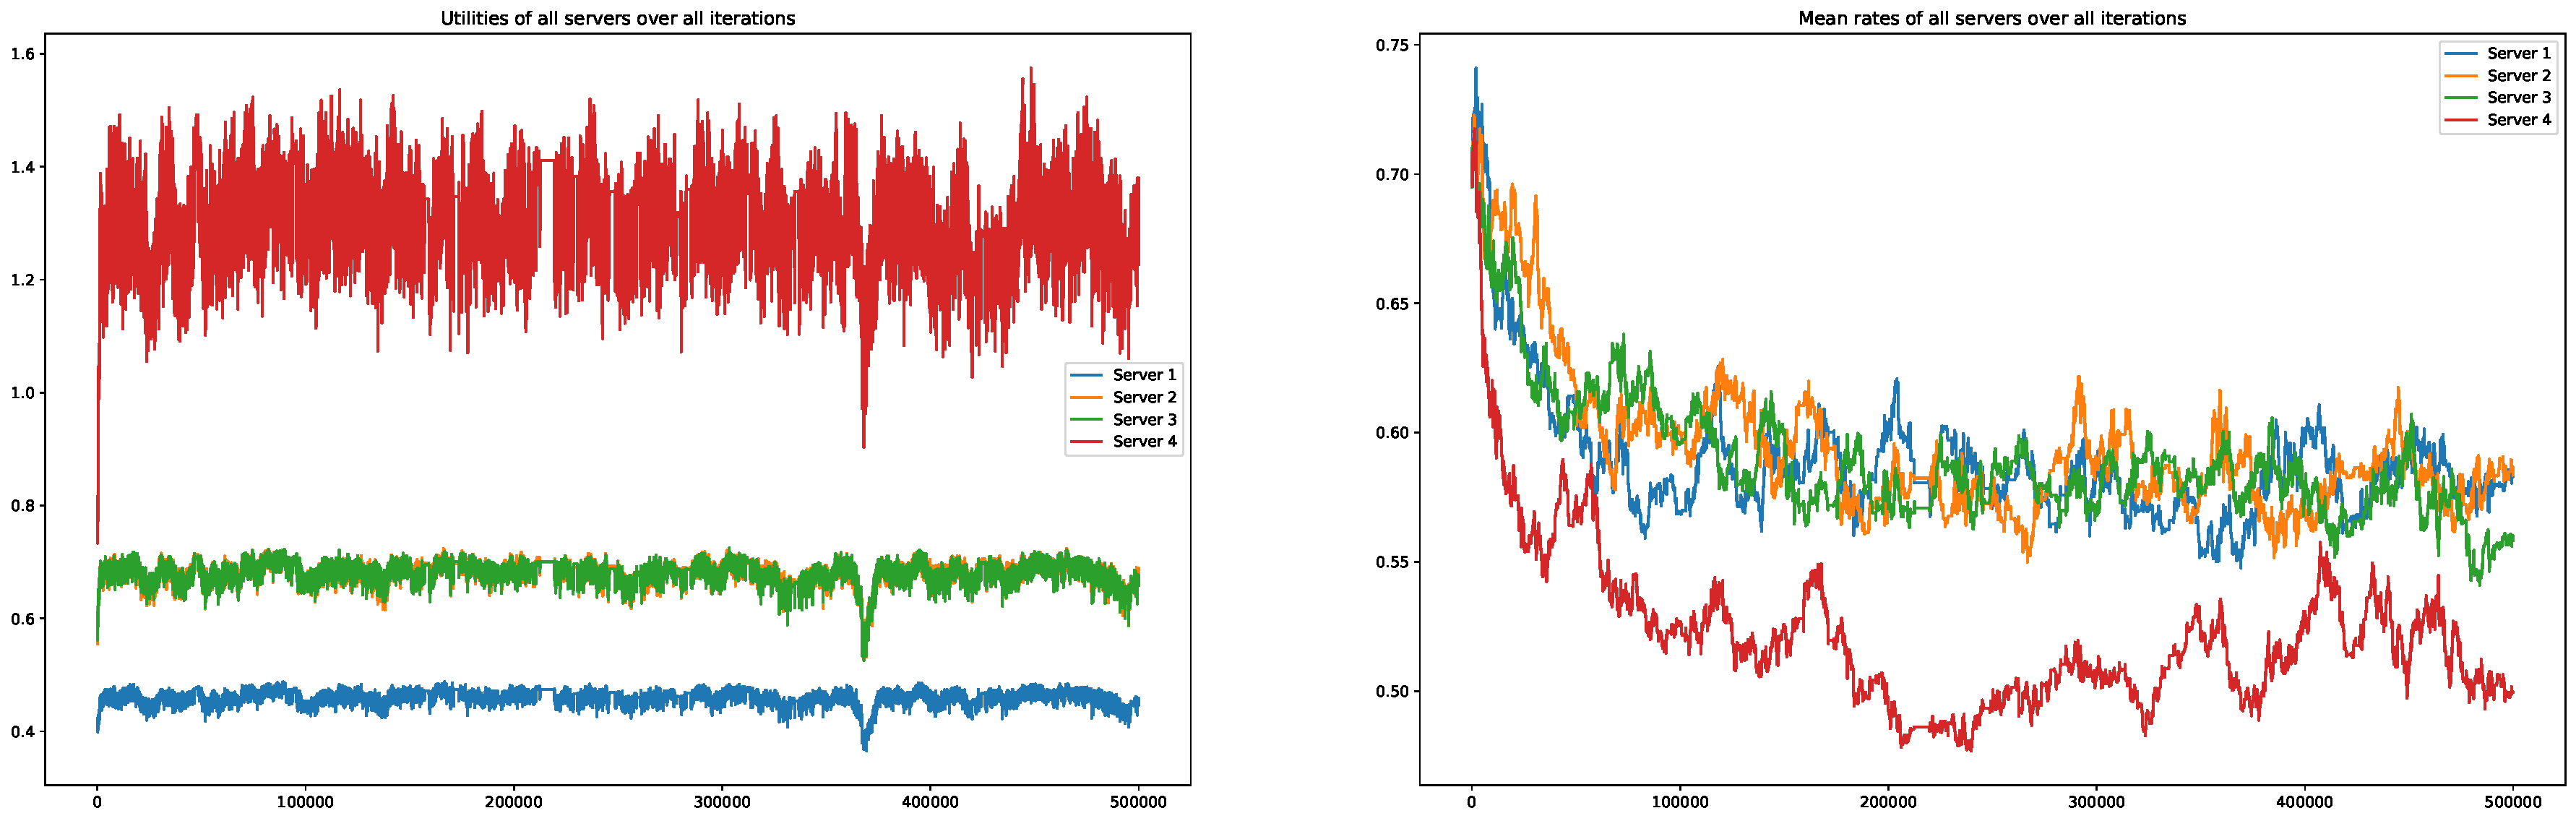
\includegraphics[width=\textwidth]{chapters/06_agent_based_extension/Bin/reinforcement_learning_results/utility_3/u3_2_e01.pdf}
    \caption{Utilities (left) and mean service rate (right) of servers from the
    reinforcement learning run using utility function \(U_k^{(3)}\) with
    \(e = 0.1\) and \(500,\!000\) time steps}
    \label{fig:RL_utility3_2_e01}
\end{figure}

Running the algorithm again for a longer runtime of \(500,\!000\) time steps
does not change the results significantly.
The same observations can be made for both figures.



\subsubsection{Utility function 7 \((U_k^{(7)})\) with \(e = 0.1\)}
\label{sec:utility_7_01_results}

Consider the plot of the mean rates of
Figures~\ref{fig:RL_utility3_1_e01}~and~\ref{fig:RL_utility3_2_e01}
(rightmost graph).
The service rate of each server consists of a different service rate for each
state \((u, v)\) of the system.
The way the reinforcement learning algorithm is constructed, the service rate
of each server is updated at each time step based on the visited states of the
system.
This means that it doesn't make sense to calculate the mean service rate from
all states of the system.
In this subsection, the weighted mean service rate is used instead, where
the weight of each state is the probability of visiting that state.
The weighted mean service rate of server \(k\) is defined as:

\begin{equation}
    \hat{\mu}^{(k)} = \sum_{(u, v) \in \mathcal{S}} \,
    \pi(u, v) \, \mu_{k, (u, v)}
\end{equation}

Consider the same example as in the previous subsection but with utility
function 7 defined in~\eqref{eq:utility_7} where
\(U_k^{(7)} = e \, \frac{I_s}{I} + (1 - e) \, \frac{R - B^{(k)}}{R}\) and
\(e = 0.1\).
Note that given the nature of this utility function the utilities of the agents
can now only be within the range \([0, 1]\).

\begin{figure}[H]
    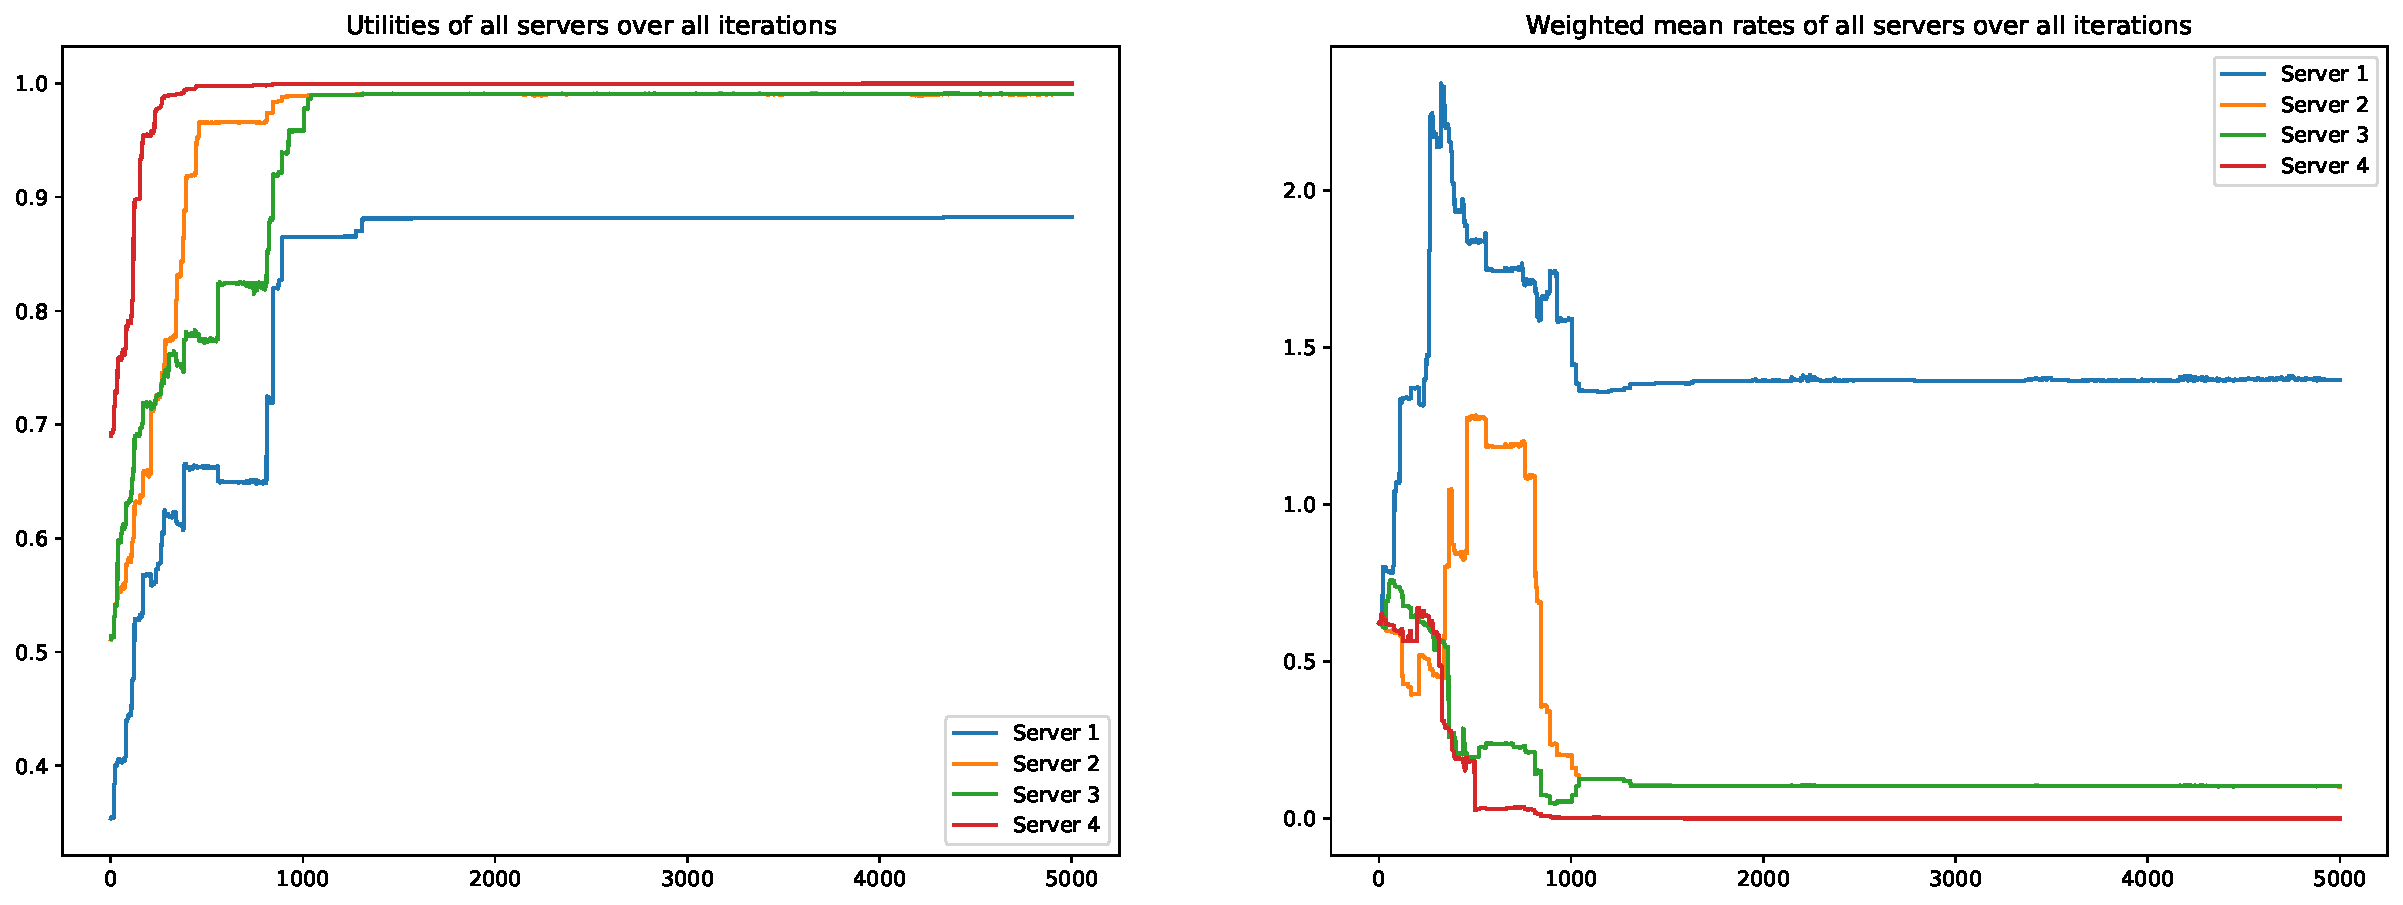
\includegraphics[width=\textwidth]{chapters/06_agent_based_extension/Bin/reinforcement_learning_results/utility_7/u7_4_e01.pdf}
    \caption{Utilities (left) and weighted mean service rate (right) of servers
    from the reinforcement learning run using utility function \(U_k^{(7)}\)
    with \(e = 0.1\).}
    \label{fig:RL_utility7_4_e01}
\end{figure}

Figure~\ref{fig:RL_utility7_4_e01} shows the utilities and weighted mean
service rate of servers from the reinforcement learning run using utility
function \(U_k^{(7)}\).
It can be seen from Figure~\ref{fig:RL_utility7_4_e01} that the utilities
follow a similar pattern to the ones from Section~\ref{sec:utility_3_results}.
That is, the utility of server \(1\) is the lowest while the utility of server
\(4\) is the highest, leaving servers \(2\) and \(3\) with similar utilities
in between.
In terms of the weighted mean service rate, servers \(2\), \(3\) and \(4\)
managed to reduce their service rate while server \(1\) had to increase its
service rate in order to maximise its utility.

What happens if the initial service rate of all servers is changed?
Would the servers manage to arrive to the same policies and same utilities?
Figure~\ref{fig:RL_utility7_4_e01_initial_02} shows the utilities and weighted
mean service rates of servers from the reinforcement learning run using utility
function \(U_k^{(7)}\) with \(e = 0.1\) and an initial service rate of
\(0.2\) for all servers.

\begin{figure}[H]
    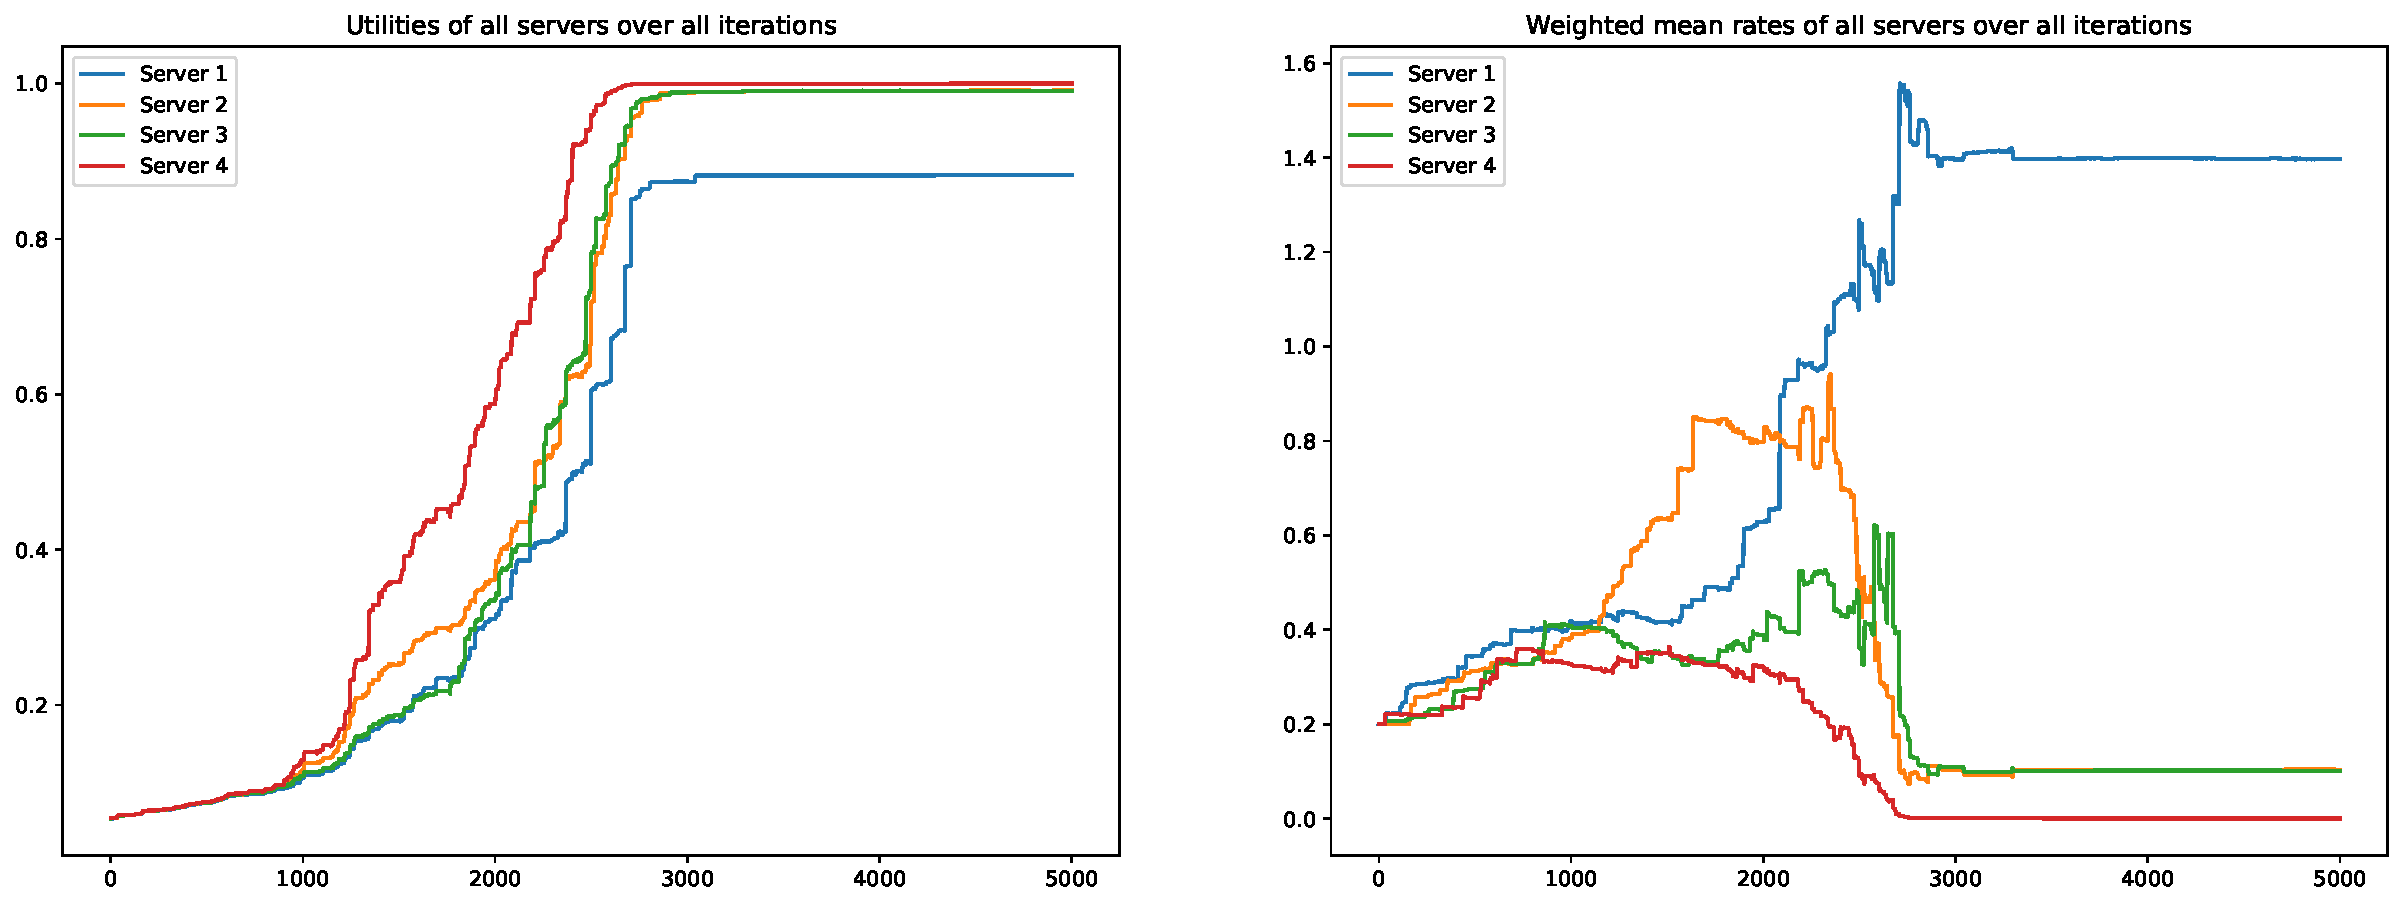
\includegraphics[width=\textwidth]{chapters/06_agent_based_extension/Bin/reinforcement_learning_results/utility_7/u7_4_e01_initial_02.pdf}
    \caption{Utilities (left) and weighted mean service rate (right) of servers
    from the reinforcement learning run using utility function \(U_k^{(7)}\)
    with \(e = 0.1\) and an initial service rate of \(0.2\) for all servers.}
    \label{fig:RL_utility7_4_e01_initial_02}
\end{figure}

Figure~\ref{fig:RL_utility7_4_e01_initial_02} shows that, even though it takes
longer to stabilise, the reinforcement learning algorithm is able to find the
same utilities as before.
In addition, it can be seen from the weighted mean service rates that servers
have also managed to find the same policies as before.
Note that more exploration is needed from the agents in order to reach the
same policies as before.

Now, consider the scenario where the initial service rate of all servers is
increased.
Figure~\ref{fig:RL_utility7_4_e01_initial_15} shows the utilities and weighted
mean service rates of servers from the reinforcement learning run using utility
function \(U_k^{(7)}\) with \(e = 0.1\) and an initial service rate of
\(1.5\) for all servers.

\begin{figure}[H]
    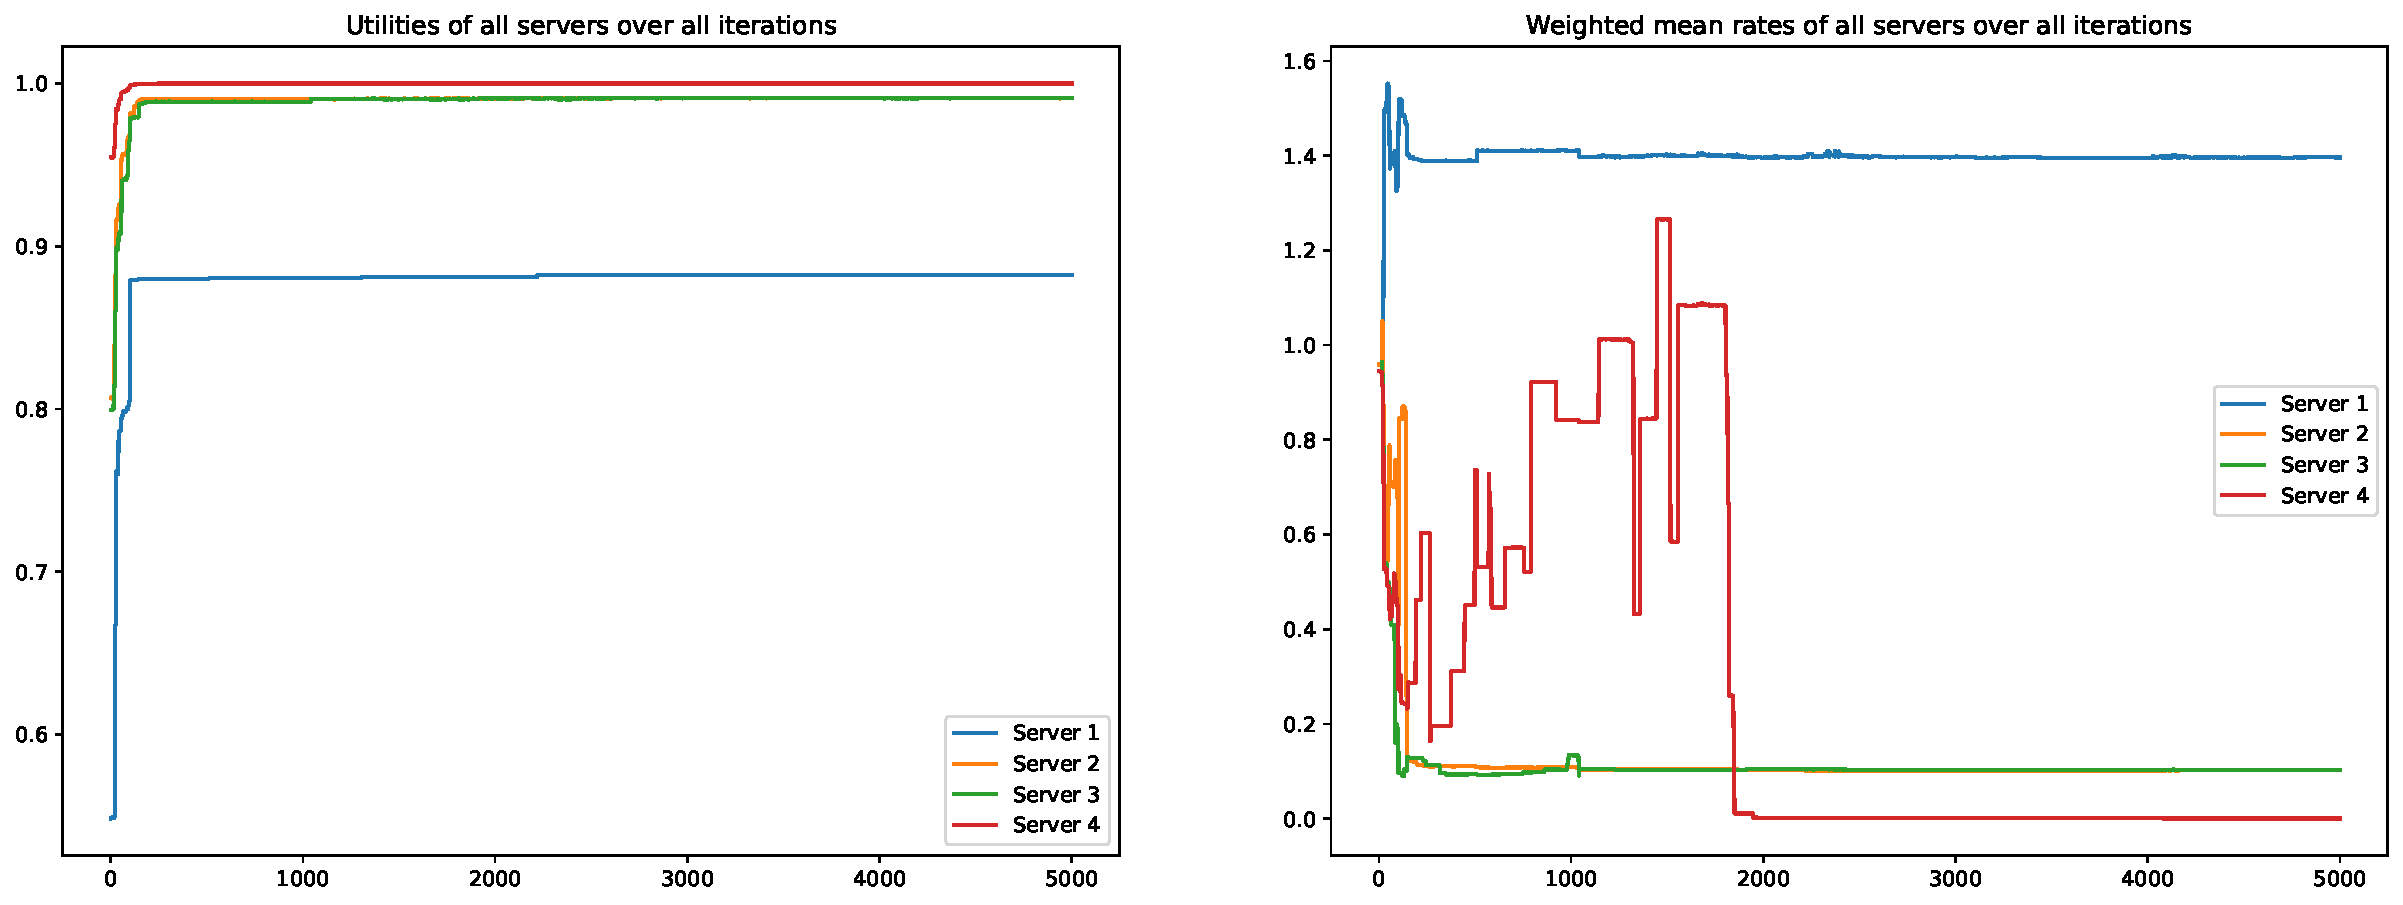
\includegraphics[width=\textwidth]{chapters/06_agent_based_extension/Bin/reinforcement_learning_results/utility_7/u7_4_e01_initial_15.pdf}
    \caption{Utilities (left) and weighted mean service rate (right) of servers
    from the reinforcement learning run using utility function \(U_k^{(7)}\)
    with \(e = 0.1\) and an initial service rate of \(1.5\) for all servers.}
    \label{fig:RL_utility7_4_e01_initial_15}
\end{figure}





\subsubsection{Utility function 7 \((U_k^{(7)})\) with e = 0.5}
\label{sec:utility_7_05_results}

This subsection considers the same parameters and utility function as in
Section~\ref{sec:utility_7_01_results} but with a different value for
parameter \(e\).
Figure~\ref{fig:RL_utility7_4_e05} shows the utilities and weighted mean
service rates of servers from the reinforcement learning run using utility
function \(U_k^{(7)}\) with \(e = 0.5\).

\begin{figure}[H]
    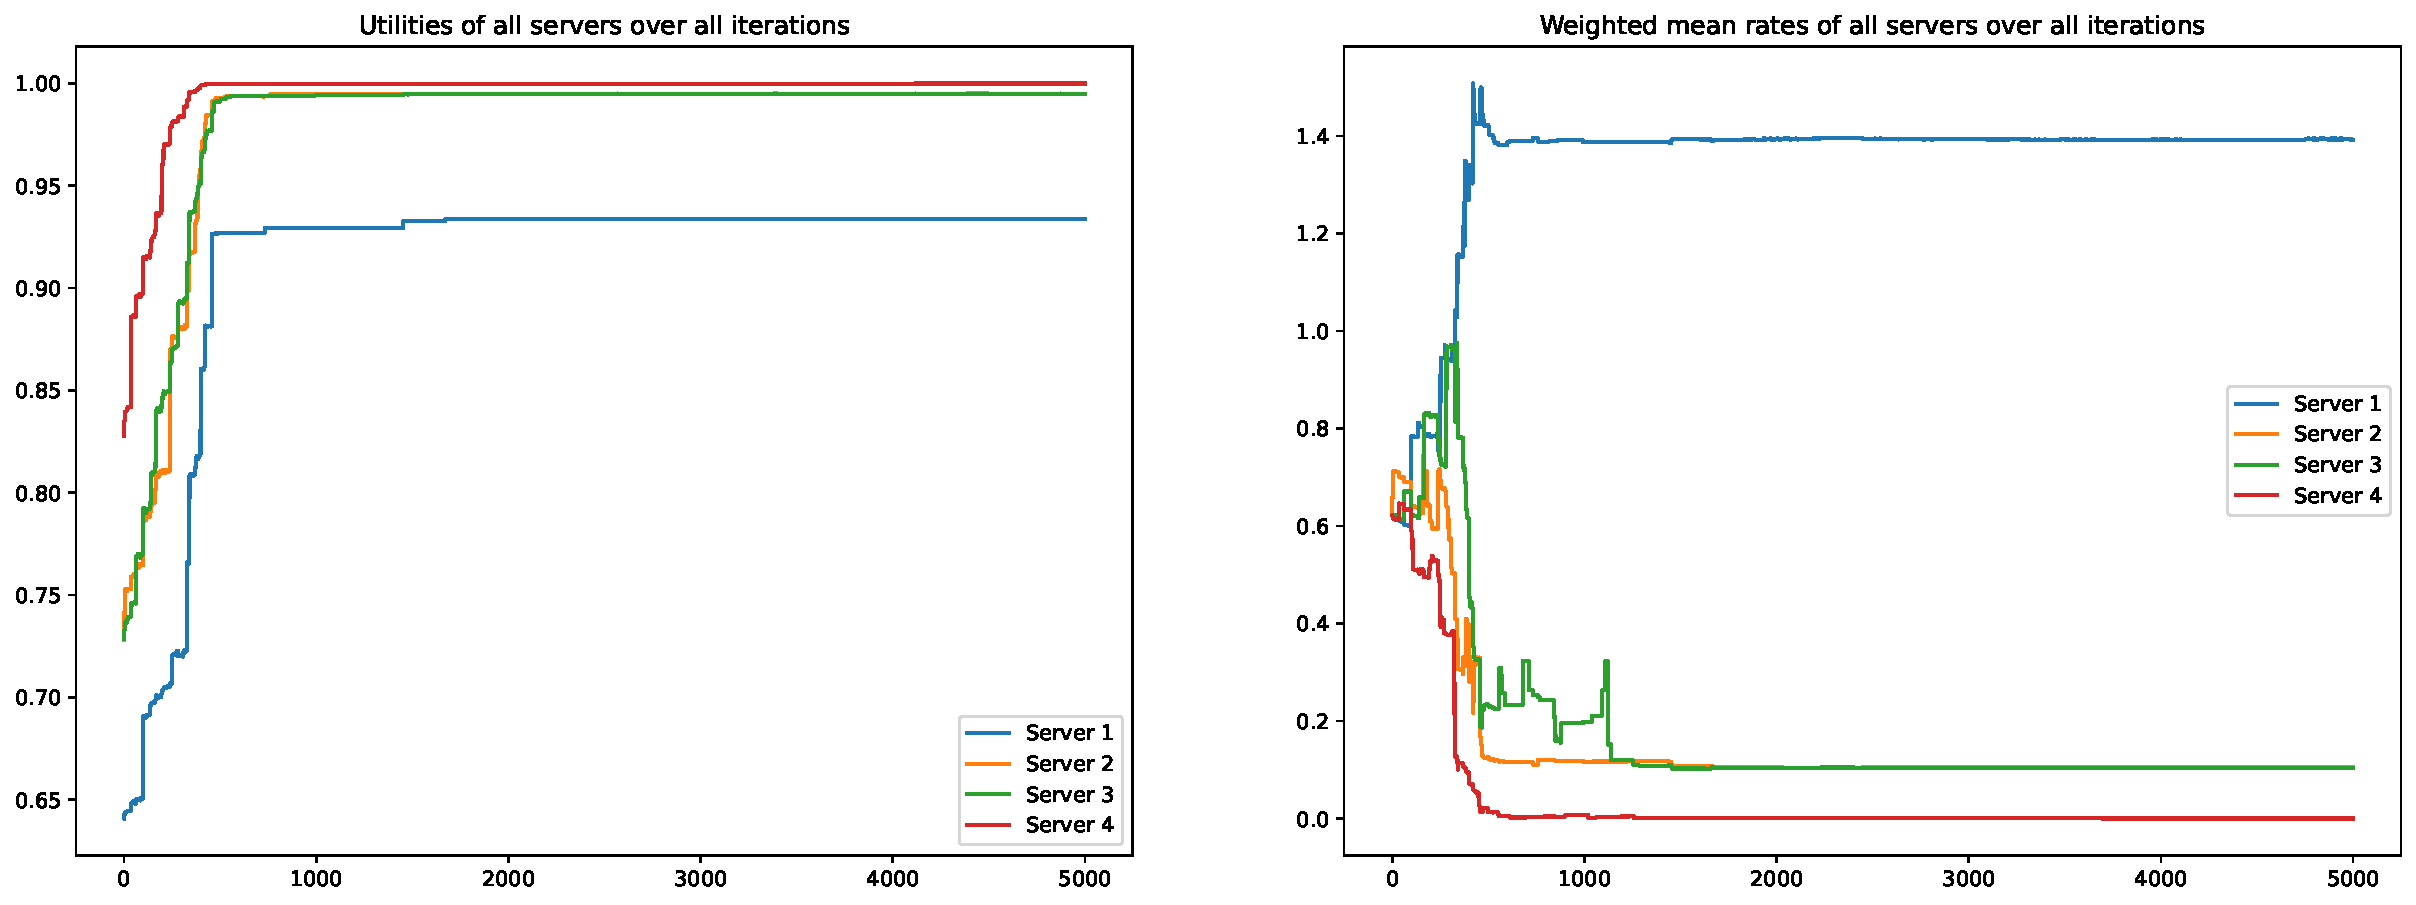
\includegraphics[width=\textwidth]{chapters/06_agent_based_extension/Bin/reinforcement_learning_results/utility_7/u7_4_e05.pdf}
    \caption{Utilities (left) and weighted mean service rate (right) of servers
    from the reinforcement learning run using utility function \(U_k^{(7)}\)
    with \(e = 0.5\).}
    \label{fig:RL_utility7_4_e05}
\end{figure}

A similar pattern to the one in Figure~\ref{fig:RL_utility7_4_e01} can be seen
from Figure~\ref{fig:RL_utility7_4_e05}.
The policies found by the agents at the end of the run are similar to the ones
found when using \(e = 0.1\).
The only difference is that the utilities are slightly higher when using
\(e = 0.5\).

Consider the scenario where the arrival rates of the two servers are increased.
Figure~\ref{fig:RL_utility7_4_e05_Lambda_45} shows the utilities and weighted
mean service rates of servers when increasing arrival rates of
\(\lambda_1 = 2\) and \(\lambda_2 = 2.5\).

\begin{figure}[H]
    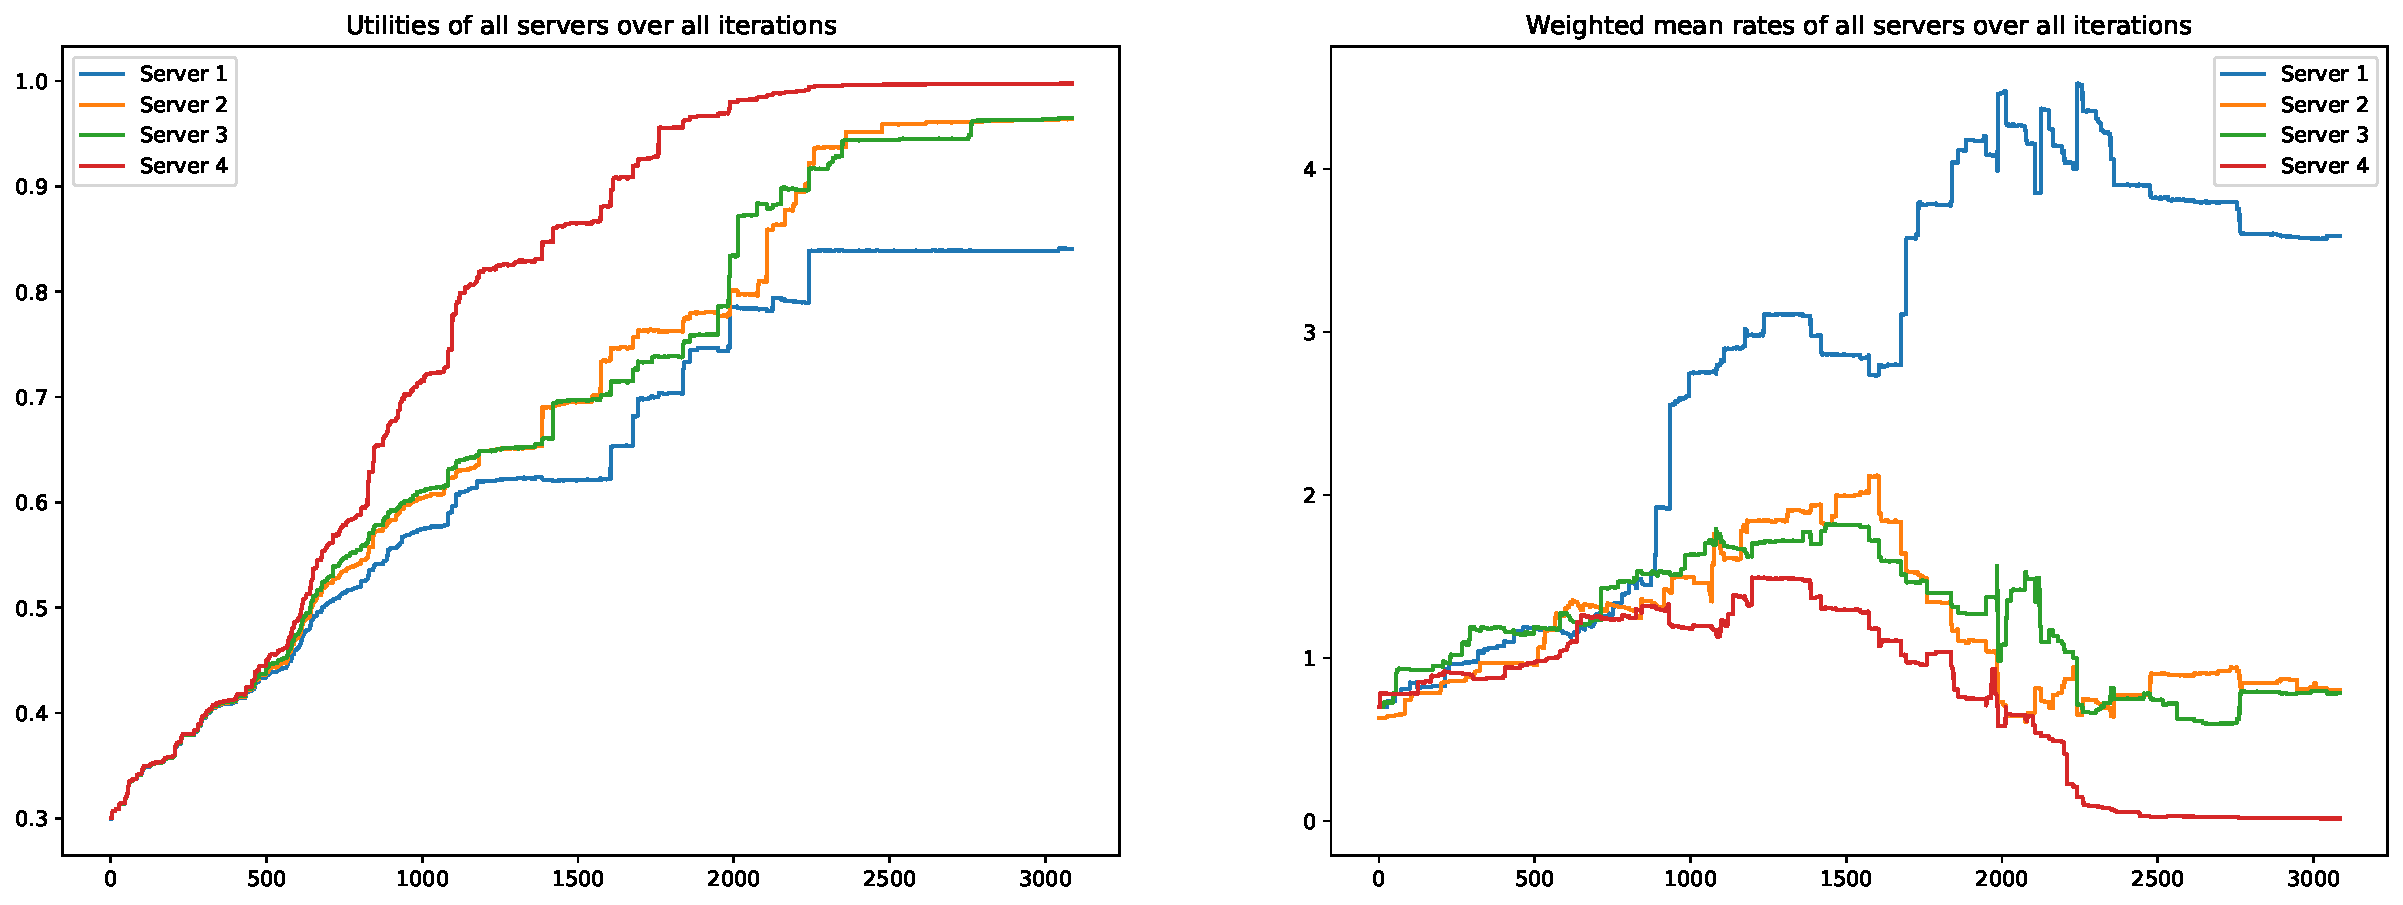
\includegraphics[width=\textwidth]{chapters/06_agent_based_extension/Bin/reinforcement_learning_results/utility_7/u7_4_e05_Lambda_45.pdf}
    \caption{Utilities (left) and weighted mean service rate (right) of servers
    from the reinforcement learning run using utility function \(U_k^{(7)}\)
    with \(e = 0.5\) and increased arrival rates of \(\lambda_1 = 2\) and
    \(\lambda_2 = 2.5\).}
    \label{fig:RL_utility7_4_e05_Lambda_45}
\end{figure}


\subsubsection{Utility function 7 \((U_k^{(7)})\) with no upper bounds}
\label{sec:utility_7_no_upper_bound_results}

Numeric results of Sections~\ref{sec:utility_3_results},
\ref{sec:utility_7_01_results} and \ref{sec:utility_7_05_results} use an upper
bound for the service rate of servers.
In other words, the service rate of servers is bounded by a specific value
so that the agents don't end up with a service rate of a really high
unrealistic value.
An example of the reinforcement learning run using utility function
\(U_k^{(7)}\) with \(e = 0.5\) and no upper bound on the service rate is
shown in Figure~\ref{fig:RL_utility7_5_no_max_e05}.

\begin{figure}[H]
    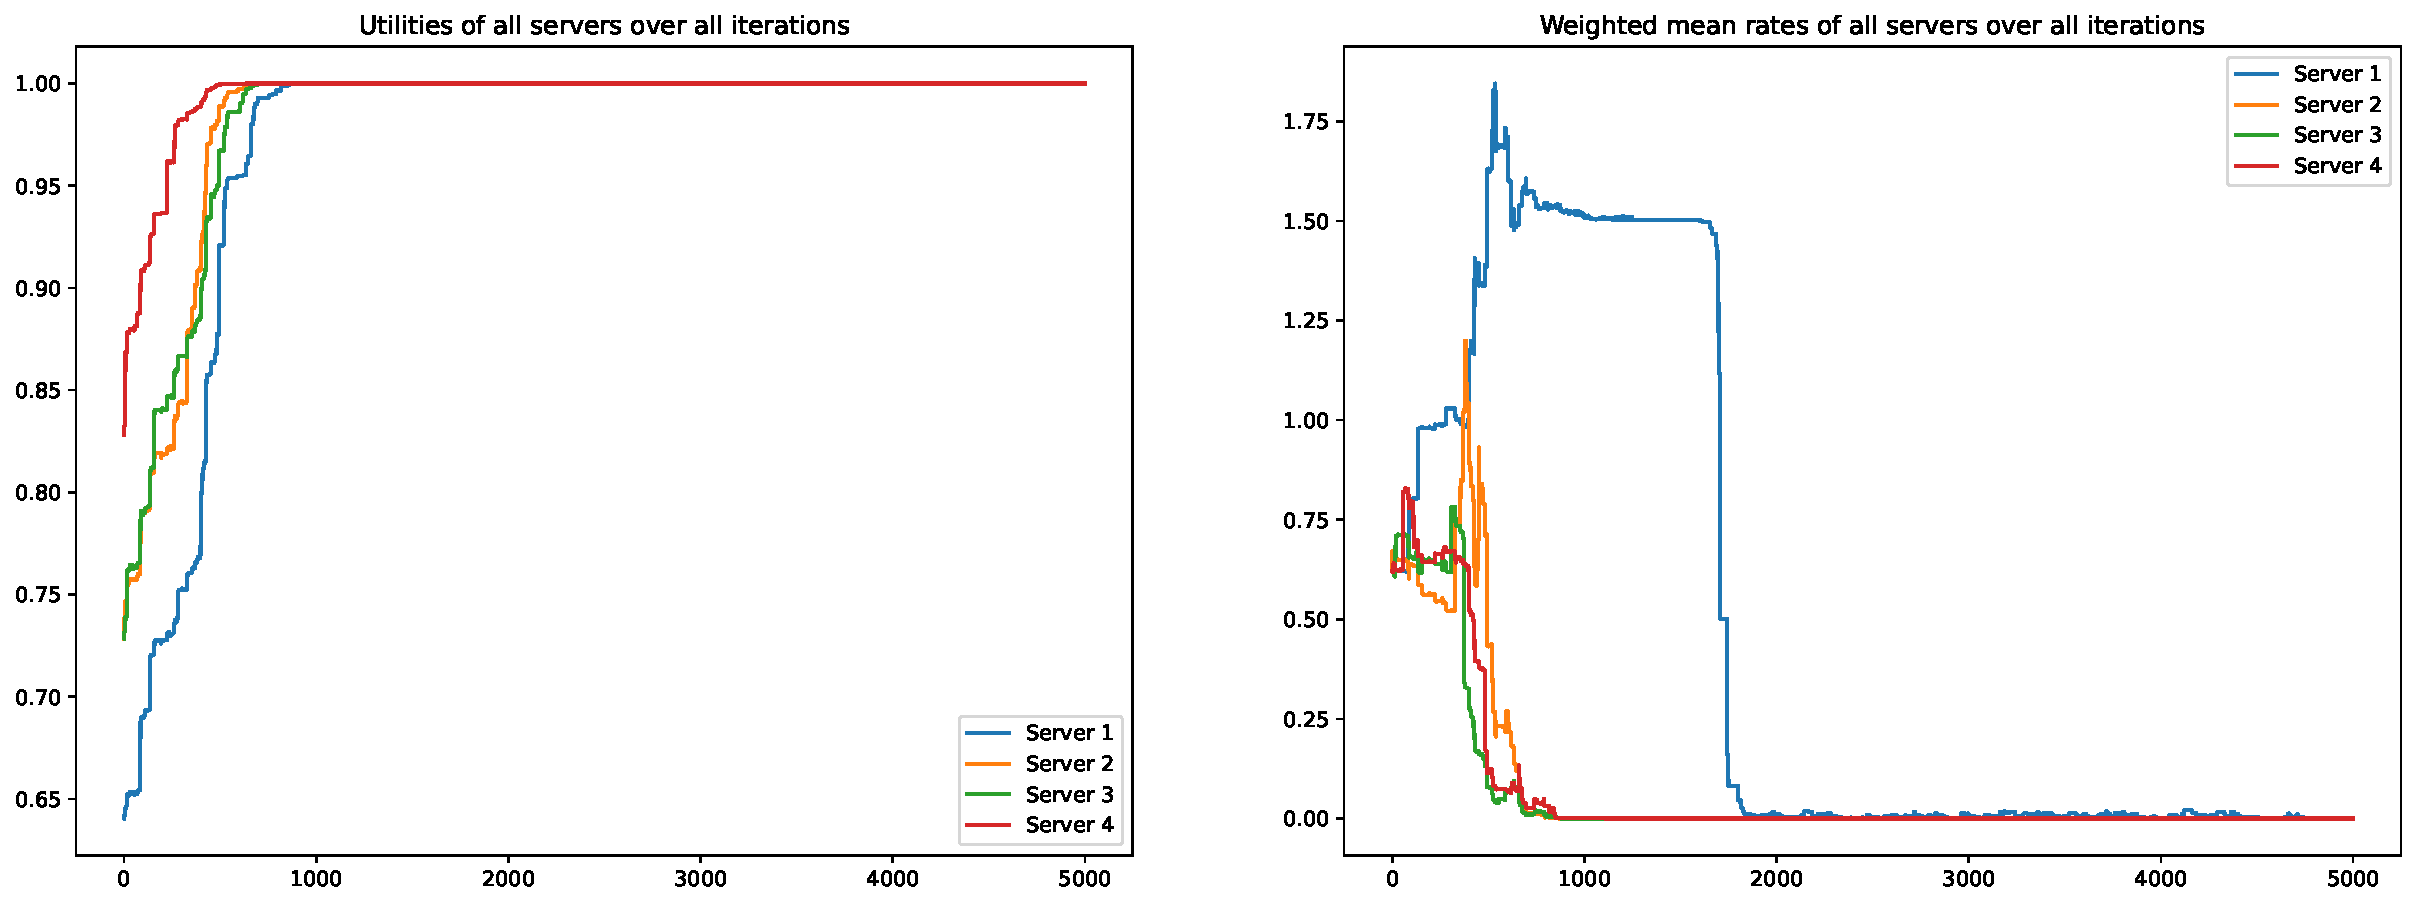
\includegraphics[width=\textwidth]{chapters/06_agent_based_extension/Bin/reinforcement_learning_results/utility_7/u7_5_no_max_e05.pdf}
    \caption{Utilities (left) and weighted mean service rate (right) of servers
    from the reinforcement learning run using utility function \(U_k^{(7)}\)
    with \(e = 0.5\) and no upper bound on the service rate.}
    \label{fig:RL_utility7_5_no_max_e05}
\end{figure}

It can be seen from Figure~\ref{fig:RL_utility7_5_no_max_e05} that the
reinforcement learning algorithm ends up with a weighted mean service rate of
servers of \(0\) while getting all their utilities to the maximum value of
\(1\).
The question to be asked is how something like this is possible.
The answer is that since the service rate of servers is not bounded, server
\(1\) ends up having a ridiculously high service rate.
The service rates of the remaining servers don't matter since every individual
that arrives, is served by server \(1\) almost instantly and leaves the system
immediately.
This results in the state probabilities being \(0\) in every state except state
\(0,0\).
In fact, only states \(0,0\) and \(0,1\) are visited in the system, where
\(0,1\) is visited for a short time because of how fast server \(1\) is
serving individuals.


\scriptsize
\begin{equation}\label{eq:no_upper_bound_states_example}
\begin{bmatrix}
    1.0 & 2.44\times10^{-19} & \text{NaN} & \text{NaN} & \text{NaN} & \text{NaN}
    & \text{NaN} & \text{NaN} & \text{NaN} & \text{NaN} & \text{NaN} \\
    \text{NaN} & \text{NaN} & \text{NaN} & \text{NaN} & \text{NaN} & \text{NaN}
    & \text{NaN} & \text{NaN} & \text{NaN} & \text{NaN} & \text{NaN} \\
    \text{NaN} & \text{NaN} & \text{NaN} & \text{NaN} & \text{NaN} & \text{NaN}
    & \text{NaN} & \text{NaN} & \text{NaN} & \text{NaN} & \text{NaN} \\
    \text{NaN} & \text{NaN} & \text{NaN} & \text{NaN} & \text{NaN} & \text{NaN}
    & \text{NaN} & \text{NaN} & \text{NaN} & \text{NaN} & \text{NaN} \\
    \text{NaN} & \text{NaN} & \text{NaN} & \text{NaN} & \text{NaN} & \text{NaN}
    & \text{NaN} & \text{NaN} & \text{NaN} & \text{NaN} & \text{NaN} \\
    \text{NaN} & \text{NaN} & \text{NaN} & \text{NaN} & \text{NaN} & \text{NaN}
    & \text{NaN} & \text{NaN} & \text{NaN} & \text{NaN} & \text{NaN} \\
    \text{NaN} & \text{NaN} & \text{NaN} & \text{NaN} & \text{NaN} & \text{NaN}
    & \text{NaN} & \text{NaN} & \text{NaN} & \text{NaN} & \text{NaN} \\
    \text{NaN} & \text{NaN} & \text{NaN} & \text{NaN} & \text{NaN} & \text{NaN}
    & \text{NaN} & \text{NaN} & \text{NaN} & \text{NaN} & \text{NaN} \\
\end{bmatrix}
\end{equation}

\begin{equation}\label{eq:no_upper_bound_rates_example}
\begin{bmatrix}
    0 & 4\times10^{15} & 9.4 & 0.5 & 2.1 & 1.8 & 0.8 & 0.4 & 0.7 & 0.7 & 0.7 \\
    \text{NaN} & \text{NaN} & \text{NaN} & \text{NaN} & \text{NaN} & \text{NaN}
    & \text{NaN} & 0.7 & 1.9 & 0.08 & 0.7 \\
    \text{NaN} & \text{NaN} & \text{NaN} & \text{NaN} & \text{NaN} & \text{NaN}
    & \text{NaN} & 1.6 & 0.7 & 0.1 & 0.7 \\
    \text{NaN} & \text{NaN} & \text{NaN} & \text{NaN} & \text{NaN} & \text{NaN}
    & \text{NaN} & 1.3 & 0.7 & 0.7 & 0.7 \\
    \text{NaN} & \text{NaN} & \text{NaN} & \text{NaN} & \text{NaN} & \text{NaN}
    & \text{NaN} & 0.7 & 0.2 & 0.7 & 0.7 \\
    \text{NaN} & \text{NaN} & \text{NaN} & \text{NaN} & \text{NaN} & \text{NaN}
    & \text{NaN} & 0.7 & 0.7 & 0.7 & 0.7 \\
    \text{NaN} & \text{NaN} & \text{NaN} & \text{NaN} & \text{NaN} & \text{NaN}
    & \text{NaN} & 0.7 & 0.7 & 0.7 & 0.7 \\
    \text{NaN} & \text{NaN} & \text{NaN} & \text{NaN} & \text{NaN} & \text{NaN}
    & \text{NaN} & 0.7 & 0.7 & 0.7 & 0.7 \\
\end{bmatrix}
\end{equation}
\normalsize

Equation~\eqref{eq:no_upper_bound_states_example} shows the state probabilities
of the system and equation~\eqref{eq:no_upper_bound_rates_example} shows the
service rates of server \(1\).
The service rates of the remaining servers are not shown since they are not
relevant.
Note that the missing values in
equation~\eqref{eq:no_upper_bound_states_example} indicate that not only the
state probabilities are \(0\) for these states, but can't even be visited by
the system.
With a service rate of \(4\times10^{15}\) for server \(1\), state
probability \(2.44\times10^{-19}\) for state \(0,1\) and state probability
\(1.0\) for state \(0,0\), the weighted mean service rate of server \(1\) is:

\begin{equation}\label{eq:no_upper_bound_mean_rate_example}
    0\times2.44\times10^{-19} + 4\times10^{15}\times1.0 \approx 0.001
\end{equation}
 
That is the reason why an upper bound on the service rates is needed.
Without an upper bound, servers could choose an extremely high service rate and
thus making the system reach unreachable scenarios.

\subsubsection{Changing arrival rates during the run}
\label{subsubsec:reinforcement_learning_special_case}

Consider once again the same parameters and utility function as in
Section~\ref{sec:utility_7_05_results}.
That is a using a utility function \(U_k^{(7)}\) with \(e = 0.5\) and arrival
rates of \(\lambda_1 = 0.5\) and \(\lambda_2 = 1\).
In this subsection the reinforcement learning algorithm is run with the same
parameters, but the arrival rates are changed during the run.
The total runtime of the reinforcement learning algorithm is 5000 time steps.
The arrival rates are set to \(\lambda_1 = 0.5\) and \(\lambda_2 = 1\) for the
first \(2000\) time steps.
Then the arrival rates are increased to \(\lambda_1 = 3\) and
\(\lambda_2 = 3.5\) for time steps \(2000\) to \(4000\) and then the arrival
rates are decreased back to \(\lambda_1 = 0.5\) and \(\lambda_2 = 1\) for the
last \(1000\) time steps.

\begin{figure}[H]
    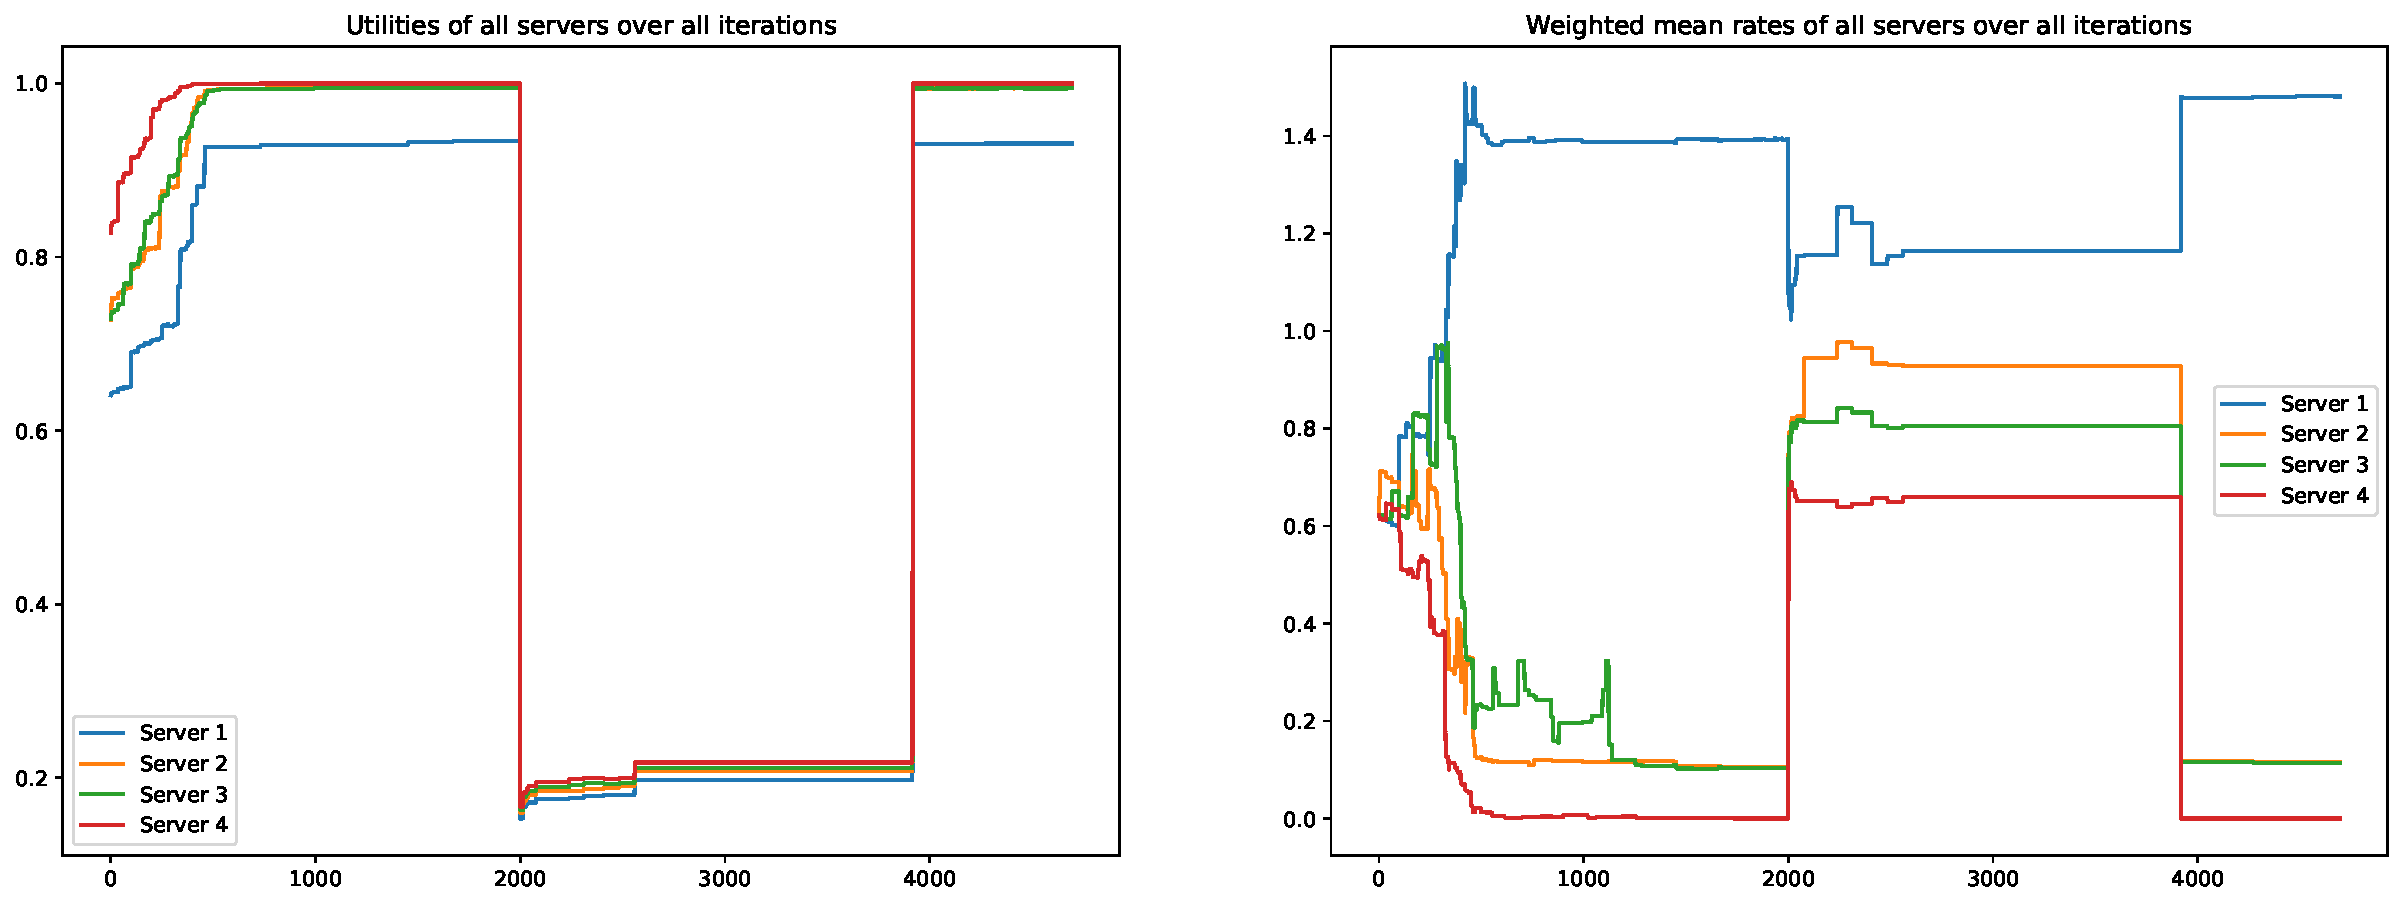
\includegraphics[width=\textwidth]{chapters/06_agent_based_extension/Bin/reinforcement_learning_results/utility_7/u7_6_final.pdf}
    \caption{Utilities (left) and weighted mean service rate (right) of servers
    from the reinforcement learning run using utility function \(U_k^{(7)}\)
    with \(e = 0.5\) and changing arrival rates throughout the run.}
    \label{fig:RL_utility7_6_final}
\end{figure}

Figure~\ref{fig:RL_utility7_6_final} shows the utilities and the weighted mean
service rates of the servers.
The first \(2000\) time steps are identical with the first \(2000\) time steps
of the reinforcement learning run of Figure~\ref{fig:RL_utility7_4_e05}.
At time step \(2000\), when the arrival rates are increased to \(\lambda_1 = 3\)
and \(\lambda_2 = 3.5\), the utilities of the agents drop significantly.
At the same time the weighted mean service rates of servers \(2\), \(3\) and
\(4\) increase significantly while server \(1\)'s rates are decreased.
In other words the arrival rates are increased so much that the priority of
the servers does not matter that much anymore.
All servers are constantly busy an they end up having more similar service
rates with each other.

At time step \(4000\) the arrival rates are decreased back to \(\lambda_1 =
0.5\) and \(\lambda_2 = 1\).
The utilities of the agents increase again and the weighted mean service rates
of servers \(2\), \(3\) and \(4\) decrease while server \(1\)'s rates are
increased.
What is more important here is how the utilities and the weighted mean service
rates change.
Having learned their optimal service rates during the first \(2000\) time steps
the servers are able to quickly retrieve their chosen service rates when the
arrival rates are decreased back to \(\lambda_1 = 0.5\) and \(\lambda_2 = 1\).
